
\section{Joint Optimization of Text and Vision}


Kimi K2.5 is a native multimodal model built upon Kimi K2 through large-scale joint pre-training on approximately 15 trillion mixed visual and text tokens. Unlike vision-adapted models that compromise either linguistic or visual capabilities, our joint pre-training paradigm enhances both modalities simultaneously. This section describes the multimodal joint optimization methodology that extends Kimi K2 to Kimi K2.5.



\subsection{Native Multimodal Pre-Training} \label{sec:joint-pre}



\begin{table}[h]
\centering
\caption{Performance comparison across different vision-text joint-training strategies. Early fusion with a lower vision ratio yields better results given a fixed total vision-text token budget.}
\begin{tabular}{lcc|cccccc}
\toprule
 & \shortstack{Vision Injection\\Timing} & \shortstack{Vision-Text\\Ratio} & \shortstack{Vision\\Knowledge} & \shortstack{Vision\\Reasoning} & \shortstack{OCR\\~} & \shortstack{Text\\Knowledge} & \shortstack{Text\\Reasoning} & \shortstack{Code\\~} \\
\midrule
Early & 0\% & 10\%:90\% & \textbf{25.8} & \textbf{43.8} & \textbf{65.7} & \textbf{45.5} & 58.5 & \textbf{24.8} \\
Mid   & 50\% & 20\%:80\% & 25.0 & 40.7 & 64.1 & 43.9 & \textbf{58.6} & 24.0 \\
Late  & 80\% & 50\%:50\% & 24.2 & 39.0 & 61.5 & 43.1 & 57.8 & 24.0 \\
\bottomrule
\end{tabular}
\label{tab:joint-train}
\end{table}


A key design question for multimodal pre-training is: Given a fixed vision-text token budget, what is the optimal vision-text joint-training strategy. Conventional wisdom~\citep{bai2025qwen3vltechnicalreport,guo2025seed15vltechnicalreport} suggests introducing vision tokens predominantly in the later stages of LLM training at high ratios (e.g., 50\% or higher) should accelerate multimodal capability acquisition, treating multimodal capability as a post-hoc add-on to linguistic competence.


However, our experiments (as shown in Table~\ref{tab:joint-train} Figure~\ref{fig:joint-train}) reveal a different story. We conducted ablation studies varying the vision ratio and vision injection timing while keeping the total vision and text token budgets fixed. To strictly meet the targets for different ratios, we pre-trained the model with text-only tokens for a specifically calculated number of tokens before introducing vision data. Surprisingly, we found that the vision ratio has minimal impact on final multimodal performance. In fact, \textbf{early fusion with a lower vision ratio yields better results given a fixed total vision-text token budget}. 
This motivates our native multimodal pre-training strategy: rather than aggressive vision-heavy training concentrated at the end, we adopt a moderate vision ratio integrated early in the training process, allowing the model to naturally develop balanced multimodal representations while benefiting from extended co-optimization of both modalities.

\subsection{Zero-Vision SFT}

Pretrained VLMs do not naturally perform vision-based tool-calling, which poses a cold-start problem for multimodal RL. Conventional approaches address this issue through manually annotated or prompt-engineered chain-of-thought (CoT) data~\citep{bai2025qwen3vltechnicalreport}, but such methods are limited in diversity, often restricting visual reasoning to simple diagrams and primitive tool manipulations (\texttt{crop}, \texttt{rotate}, \texttt{flip}).

An observation is that high-quality text SFT data are relatively abundant and diverse.
We propose a novel approach, zero-vision SFT, that uses only text SFT data to activate the visual, agentic capabilities during post-training.
In this approach, all image manipulations are proxied through programmatic operations in \texttt{IPython}, effectively serving as a generalization of traditional vision tool-use. This "zero-vision" activation enables diverse reasoning behaviors, including pixel-level operations such as object size estimation via binarization and counting, and generalizes to visually grounded tasks such as object localization, counting, and OCR. 

Figure~\ref{fig:visionzerorl_curves} illustrates the RL training curves, where the starting points are obtained from zero-vision SFT. The results show that zero-vision SFT is sufficient for activating vision capabilities while ensuring generalization across modalities. This phenomenon is likely due to the joint pretraining of text and vision data as described in Section~\ref{sec:joint-pre}. Compared to zero-vision SFT, our preliminary experiments show that text-vision SFT yields much worse performance on visual, agentic tasks, possibly because of the lack of high-quality vision data.


\subsection{Joint Multimodal Reinforcement Learning (RL)}
\label{sec:native_multimodal_rl}


In this section, we describe the methodology implemented in K2.5 that enables effective multimodal RL, from outcome-based visual RL to emergent cross-modal transfer that enhances textual performance.


\begin{figure}[t]
    \centering
    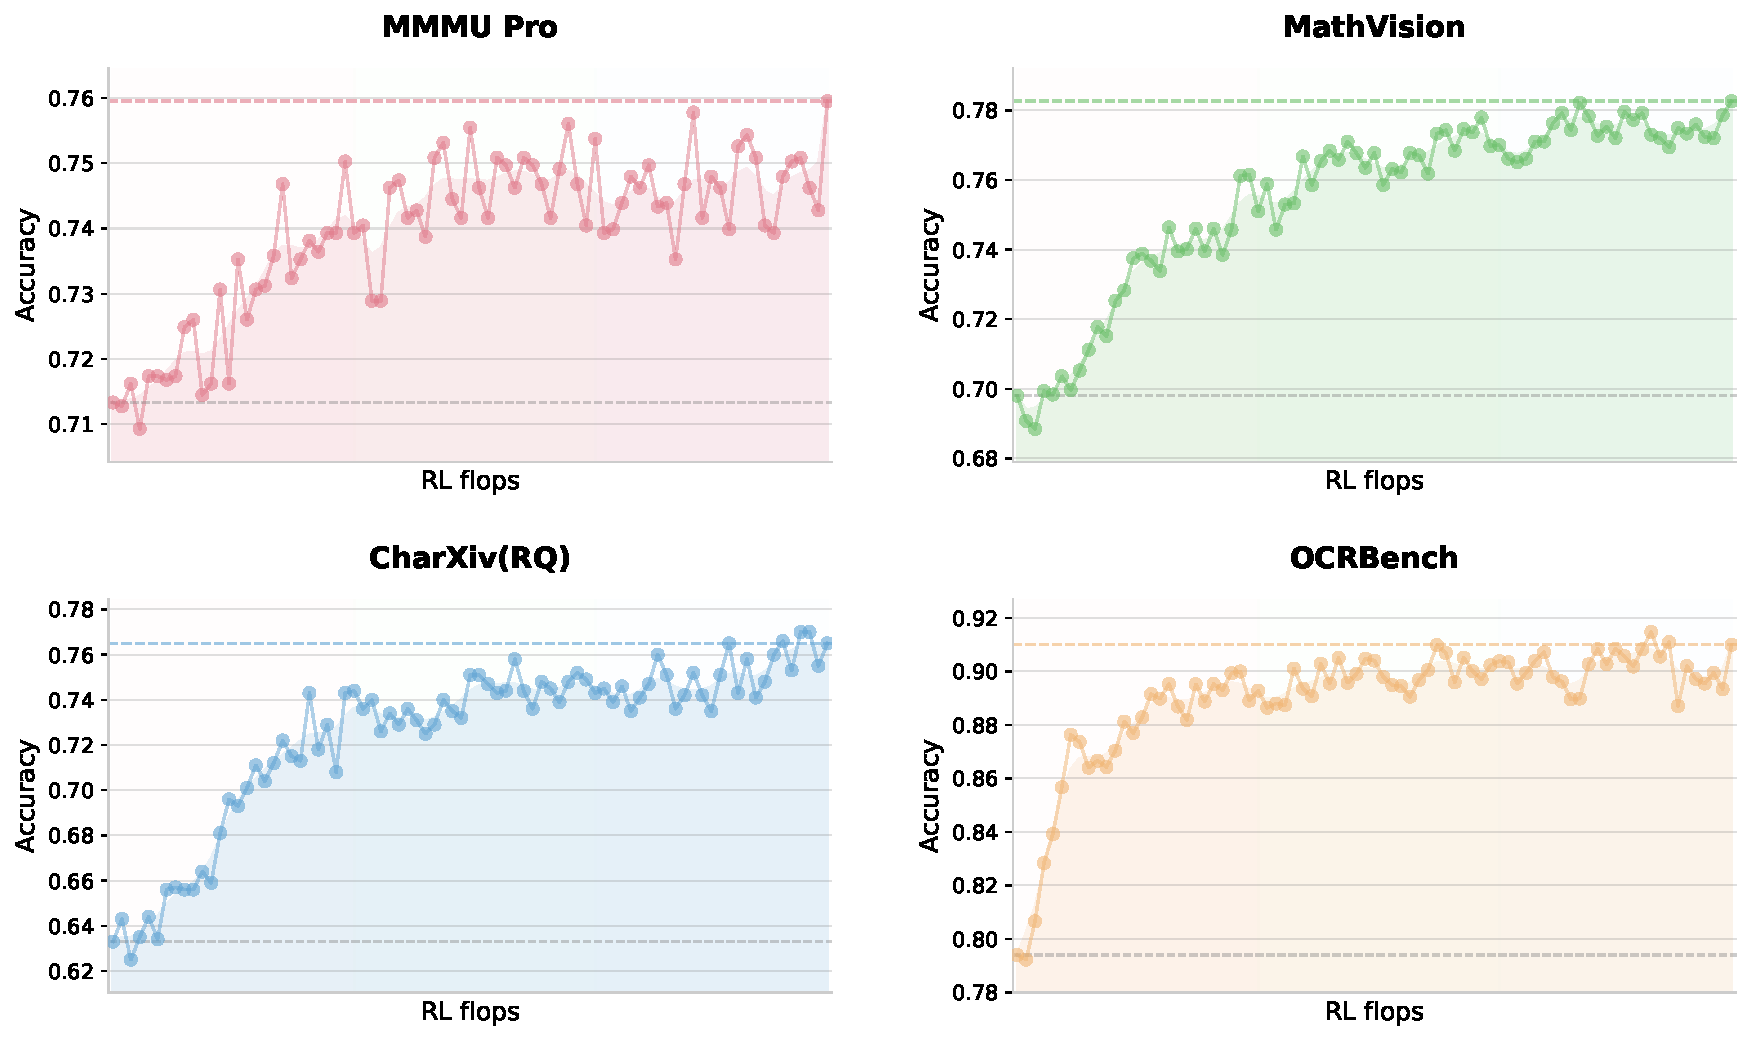
\includegraphics[width=0.9\textwidth]{figures/k25_visionzerorl_curves.pdf}
    \caption{Vision RL training curves on vision benchmarks starting from minimal zero-vision SFT. By scaling vision RL FLOPs, the performance continues to improve, demonstrating that zero-vision activation paired with long-running RL is sufficient for acquiring robust visual capabilities.} 
    \label{fig:visionzerorl_curves}
\end{figure}

\paragraph{Outcome-Based Visual RL}
Following the zero-vision SFT, the model requires further refinement to reliably incorporate visual inputs into reasoning. Text-initiated activation alone exhibits notable failure modes: visual inputs are sometimes ignored, and images may not be attended to when necessary. We employ outcome-based RL on tasks that explicitly require visual comprehension for correct solutions.
We categorize these tasks into three domains:
 \begin{itemize}
 \item \textbf{Visual grounding and counting:} Accurate localization and enumeration of objects within images;
 \item \textbf{Chart and document understanding:} Interpretation of structured visual information and text extraction;
 \item \textbf{Vision-critical STEM problems:} Mathematical and scientific questions filtered to require visual inputs.
 \end{itemize}
Outcome-based RL on these tasks improves both basic visual capabilities and more complex agentic behaviors. Extracting these trajectories for rejection-sampling fine-tuning (RFT) enables a self-improving data pipeline, allowing subsequent joint RL stages to leverage richer multimodal reasoning traces.

\paragraph{Visual RL Improves Text Performance}

\begin{table}[h]
\centering
\caption{Cross-Modal Transfer: Vision RL Improves Textual Knowledge}
\begin{tabular}{lccc}
\toprule
\textbf{Benchmark} & \textbf{Before Vision-RL} & \textbf{After Vision-RL} & \textbf{Improvement} \\
\midrule
MMLU-Pro & 84.7 & 86.4 & +1.7 \\
GPQA-Diamond & 84.3 & 86.4 & +2.1 \\
LongBench v2 & 56.7 & 58.9 & +2.2 \\
\bottomrule
\end{tabular}
\label{tab:vision_rl_text}
\end{table}

 To investigate potential trade-offs between visual and textual performance, we evaluated text-only benchmarks before and after visual RL. Surprisingly, outcome-based visual RL produced measurable improvements in textual tasks, including MMLU-Pro (84.7\% $\rightarrow$ 86.4\%), GPQA-Diamond (84.3\% $\rightarrow$ 86.4\%), and LongBench v2 (56.7\% $\rightarrow$ 58.9\%) (Table~\ref{tab:vision_rl_text}).
Analysis suggests that visual RL enhances calibration in areas requiring structured information extraction, reducing uncertainty on queries that resemble visually grounded reasoning (e.g., counting, OCR). These findings indicate that visual RL can contribute to cross-modal generalization, improving textual reasoning without observable degradation of language capabilities.

\textbf{Joint Multimodal RL} Motivated by the finding that robust visual capabilities can emerge from zero-vision SFT paired with vision RL---which further enhances general text abilities---we adopt a joint multimodal RL paradigm during Kimi K2.5's post-training. Departing from conventional modality-specific expert divisions, we organize RL domains not by input modality but by abilities---knowledge, reasoning, coding, agentic, etc. These domain experts jointly learn from both pure-text and multimodal queries, while the Generative Reward Model (GRM) similarly optimizes across heterogeneous traces without modality barriers. This pardaigm ensures that capability improvements acquired through either textual or visual inputs inherently generalize to enhance related abilities across the alternate modality, thereby maximizing cross-modal capability transfer.


